\chapter{Lexicon-grammar}
\label{chap-lexicon-grammar}
\index{Lexicon-grammar}
The tables of lexicon-grammar are a compact way for representing syntactical
properties of the elements of a language. It is possible to automatically
construct local grammars from such tables, due to a mechanism of parameterized
graphs. 

\bigskip
\noindent In the first part of the chapter the formalism of tables is presented.
The second part describes parameterized graphs and a mechanism of automatically
lexicalizing them with lexicon-grammar tables.


\section{Lexicon-grammar tables}
\index{Lexicon-grammar!tables}\index{Matrices}
Lexicon-grammar is a methodology developed by Maurice Gross and the LADL team
\index{LADL} (\cite{L}, \cite{BGL}, \cite{methodes-en-syntaxe}, \cite{GL},
\cite{gross1994}, \cite{gross1994b}, \cite{gross1991}, \cite{gross1986}, 
\cite{gross1984}, \cite{gross1984b}, \cite{gross1983}, \cite{gross1982}, 
\cite{gross1978}, \cite{leclere2005}, \cite{salkoff2004})
based on the following principle: every verb has an almost unique set of syntactical
properties. Due to this fact, these properties need to be systematically
described, since it is impossible to predict the exact behavior of a verb. These
descriptions are represented by matrices where rows correspond to verbs and
columns to syntactical properties. The considered properties are formal
properties such as the number and nature of allowed complements of the verb and
the different transformations the verb can undergo (passivization,
nominalisation, extraposition, etc.). The matrices, or tables, are mostly binary:
a \verb$+$ sign occurs at the intersection of a row and a column of a property if
the verb has that property, a \verb+-+ sign if not. \index{Syntactical
properties} More information in \url{http://infolingu.univ-mlv.fr}, including
some lexicon-grammar tables that you can freely download.

\bigskip
\noindent This type of description has also been applied to adjectives
(\cite{these-annie}), predicative nouns (\cite{les-nominalisations},
\cite{les-predicats-nominaux}, \cite{giry1978}, \cite{gross1976},
\cite{ranchhod2001}), 
adverbs (\cite{syntaxe-de-ladverbe},
\cite{grammaire-des-adverbes}), as well as frozen expressions, in many languages
(\cite{lexique-grammaire-allemand2}, \cite{lexique-grammaire-italien2},
\cite{lexique-grammaire-italien}, \cite{lexique-grammaire-coreen2},
\cite{lexique-grammaire-coreen}, \cite{lexique-grammaire-malgache},
\cite{lexique-grammaire-espagnol}, \cite{lexique-grammaire-allemand},
\cite{lexique-grammaire-hongrois}, \cite{ranchhod1996}, \cite{ranchhod1991},
\cite{gross1986b}).

\bigskip
\noindent Figure \ref{fig-table-32NM} shows an example of a lexicon-grammar table.
The table contains verbs that, among other definitional properties, do not admit
passivization.

\begin{figure}[!ht]
\begin{center}
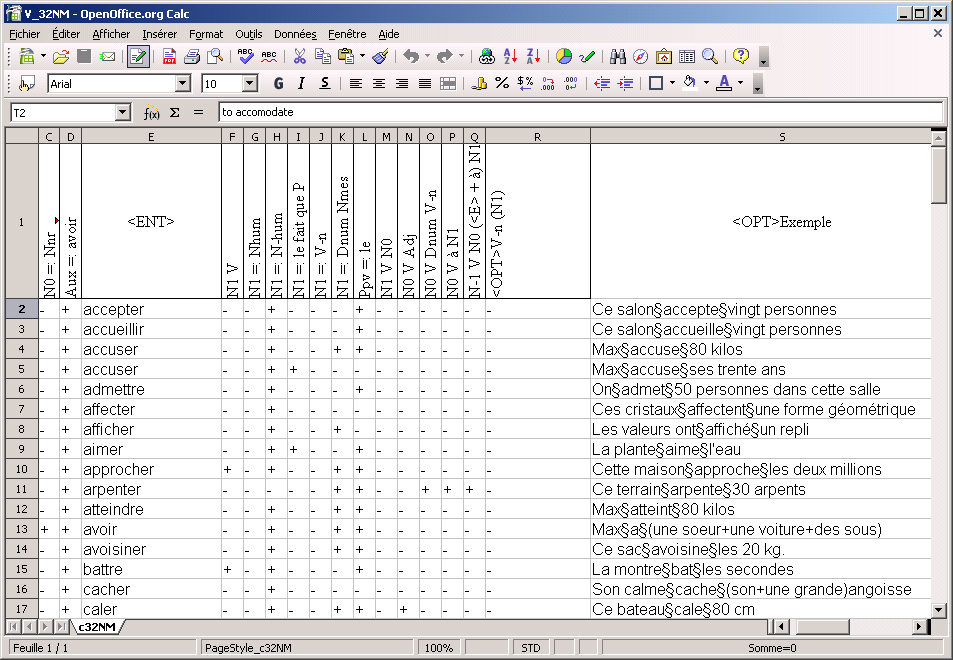
\includegraphics[width=15cm]{resources/img/fig8-1.png}
\caption{Lexicon-grammar Table 32NM\label{fig-table-32NM}}
\end{center}
\end{figure}

\section{Conversion of a table into graphs}
\subsection{Principle of parameterized graphs}
\index{Parameterized graphs}\index{Graph!parameterized}
The conversion of a table into graphs is carried out by a mechanism involving
parameterized graphs. The principle is the following: a graph that describes the
possible constructions is constructed manually. That graphs refers to the columns
of the table in the form of parameters or variables. Afterwards, for each line of
the table a copy of this graph is constructed where the variables are replaced
with the contents of the cell at the intersection of line and the column that
corresponds to the variable. If a cell of the table contains the \verb$+$ sign,
the corresponding variable is replaced by \verb+<E>+. If the cell contains the
\verb+-+ sign,  the box containing the corresponding variable is removed,
interrupting the paths through that box. In all other cases the variable is
replaced by the contents of the cell.


\subsection{Format of the table}
The lexicon-grammar tables are usually encoded with the aid of a spreadsheet like
OpenOffice.org Calc (\cite{OpenOffice}). To be usable with Unitex, the
tables have to be encoded in Unicode text format in accordance with the following
convention: the columns need to be separated by a tab and the lines by a newline.

\bigskip
\noindent In order to convert a table with OpenOffice.org Calc, save it in text
format (\verb$.csv$ extension). You can then parameterize the output format with a
window as shown on Figure \ref{fig-csv-export}. Choose "Unicode", select
tabulation as column separator and do not set any text delimiter.

\begin{figure}[!ht]
\begin{center}
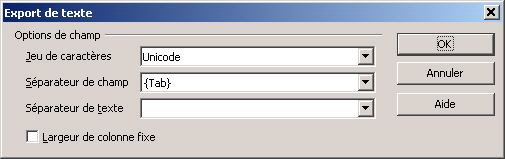
\includegraphics[width=12cm]{resources/img/fig8-2.png}
\caption{Saving a table with OpenOffice.org Calc\label{fig-csv-export}}
\end{center}
\end{figure}

\bigskip
\noindent During the generation of the graphs, Unitex skips the first line, 
considering that it
contains the headings of the columns. It is therefore necessary to ensure that
the headings of the columns occupy exactly one line. If there is no line for the
heading, the first line of a table will be ignored anyway, and if there are
multiple heading lines, from the second line on they will be interpreted as lines
of the table.


\subsection{Parameterized graphs}
Parameterized graphs are graphs with variables referring to the columns of a
lexicon-grammar table. This mechanism is usually used with syntactic
graphs, but nothing prevents the construction of parameterized graphs for
inflection, preprocessing, or for normalization.

\index{Variables!in parameterized graphs}
\bigskip
\noindent Variables that refer to columns are formed with the \verb+@+ symbol
\index{\verbc{"@}} followed by the name of the column in capital letters (the
columns are named starting with \verb+A+).

\bigskip
\noindent Example: \verb+@C+ refers to the third column of the table.

\bigskip
\noindent Whenever a variable takes the value of a \verb$+$ or \verb+-+ sign, the
\verb+-+ sign corresponds to the removal of a path through that variable. It is
possible to swap the meaning of these signs by typing an exclamation mark in
front of the \verb+@+ symbol. In that case, the path is removed when there is a
\verb$+$ sign and kept where there is a \verb+-+ one. In all other cases, the
variable is replaced by the content of the table cell.

\bigskip
\noindent The special variable \verb+@%+ \index{\verbt{"@\%}} is replaced by the
number of the line in the table. The fact that its value is different for each
line allows for its use as a simple characterization of a line. That variable is
not affected by an exclamation point to the left of it.

\bigskip
\noindent Figure \ref{fig-reference-graph} shows an example of a parameterized
graph designed to be applied to the lexicon-grammar table 31H presented in figure
\ref{fig-table-31H}.

\begin{figure}[!ht]
\begin{center}
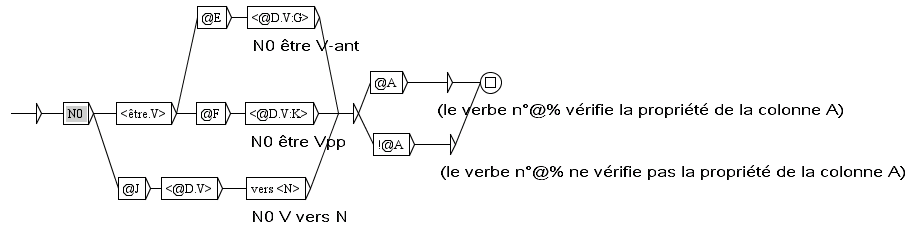
\includegraphics[width=15cm]{resources/img/fig8-3.png}
\caption{Example of parameterized graph\label{fig-reference-graph}}
\end{center}
\end{figure}

\begin{figure}[!ht]
\begin{center}
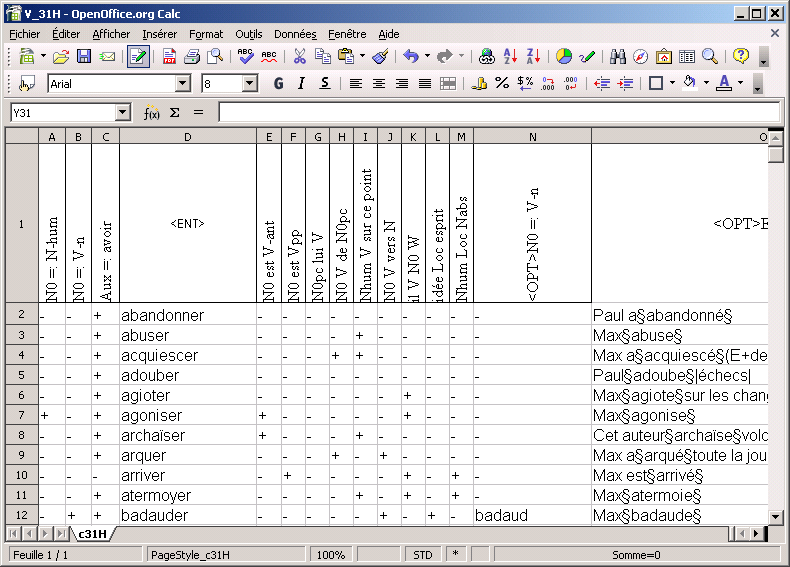
\includegraphics[width=15cm]{resources/img/fig8-4.png}
\caption{Lexicon-grammar table 31H\label{fig-table-31H}}
\end{center}
\end{figure}


\subsection{Automatic generation of graphs}
In order to be able to generate graphs from a parameterized graph and a table,
first of all the table must be opened by clicking on "Open..." in the 
"Lexicon-Grammar" menu (see figure \ref{fig-lexicon-grammar-menu}). The table
must be in Unicode text format.

\begin{figure}[!ht]
\begin{center}
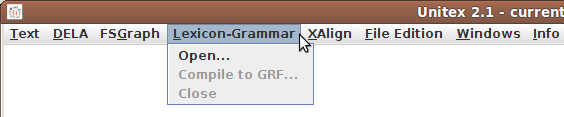
\includegraphics[width=12cm]{resources/img/fig8-5.png}
\caption{Menu "Lexicon-Grammar"\label{fig-lexicon-grammar-menu}}
\end{center}
\end{figure}

\bigskip
\noindent The selected table is then displayed in a window (see figure figure
\ref{fig-table-display}). If it does not appear on your screen, it may be
hidden by other Unitex windows.

\begin{figure}[!ht]
\begin{center}
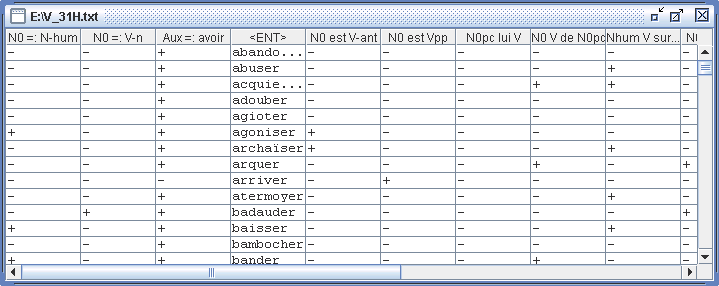
\includegraphics[width=15cm]{resources/img/fig8-6.png}
\caption{Displaying a table\label{fig-table-display}}
\end{center}
\end{figure}

\bigskip
\noindent To automatically generate graphs from a parameterized graph, click on "Compile to
GRF..." in the "Lexicon-Grammar" menu. The window in figure
\ref{fig-configuration-graph-generation} shows this.

\begin{figure}[!ht]
\begin{center}
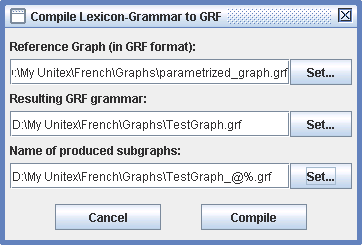
\includegraphics[width=9cm]{resources/img/fig8-7.png}
\caption{Configuration of the automatic generation of graphs\label{fig-configuration-graph-generation}}
\end{center}
\end{figure}

\bigskip
\noindent In the "Reference Graph (in GRF format)" frame, indicate the name of
the parameterized graph to be used. In the "Resulting GRF grammar" frame,
indicate the name of the main graph that will be generated. This main graph is a graph
that invokes all the graphs that are going to be generated. When launching a
search in a text with that graph, all the generated graphs are simultaneously
applied.

\bigskip
\noindent The "Name of produced subgraphs" frame is used to set the name of each
graph that will be generated. Enter a name containing \verb+@%+, because for each line of
the table, \verb+@%+ will be replaced the line number, which guarantees that each
graph name will be unique. For example, if the main graph is called
"\verb+TestGraph.grf+" and if subgraphs are called "\verb+TestGraph_@%.grf+", the
graph generated from the 16th line of the line will be named
"\verb+TestGraph_0016.grf+".

\bigskip
\noindent Figures \ref{fig-archaiser} and \ref{fig-badauder} show
two graphs generated by applying the parameterized graph of figure
\ref{fig-reference-graph} at table 31H.

\bigskip
\noindent Figure \ref{fig-main-graph} shows the resulting main graph.

\begin{figure}[!ht]
\begin{center}
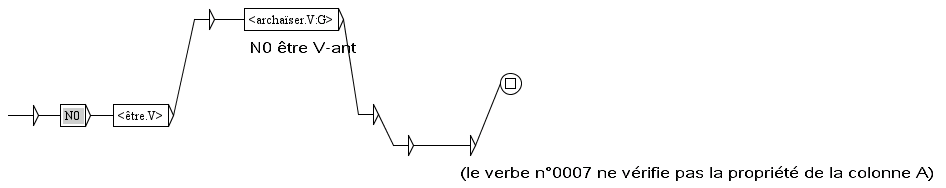
\includegraphics[width=15cm]{resources/img/fig8-8.png}
\caption{Graph generated for the verb
\texttt{archa\"iser}\label{fig-archaiser}}
\end{center}
\end{figure}

\begin{figure}[!ht]
\begin{center}
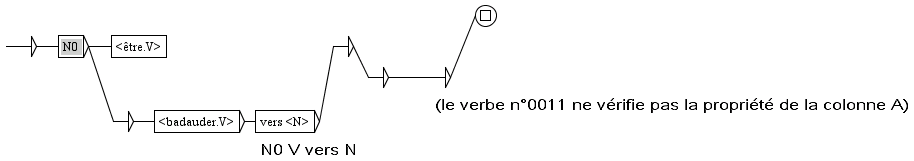
\includegraphics[width=15cm]{resources/img/fig8-9.png}
\caption{Graph generated for the verb \texttt{badauder}\label{fig-badauder}}
\end{center}
\end{figure}

\begin{figure}[!ht]
\begin{center}
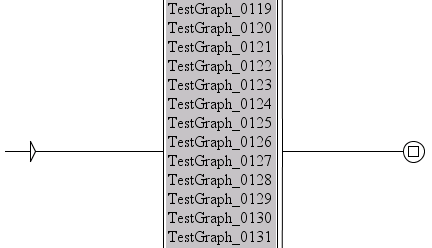
\includegraphics[width=10cm]{resources/img/fig8-10.png}
\caption{Main graph referring to all the generated
graphs\label{fig-main-graph}}
\end{center}
\end{figure}


